\textcolor{prime}{\textsf{Findings}} \\
\begin{itemize}
\item When we only use the first term of the heuristic, (equation~\ref{fig:woheu}),  the system can leave a trot gait and quickly becomes unstable at higher amplitude disturbances.

\item When we use both terms of the heuristic the system can reject higher amplitude disturbances because it is able to maintain a trot gait. 

\item System can still be forced to leave a trot gait if disturbance is large enough
\end{itemize}

\vspace{2EX}
\textcolor{prime}{\textsf{Future Work}} \\
\begin{itemize}
	\item Test the controller on a real robot to verify its rohbustness given:
	\begin{itemize}
		\item motor dynamics
		\item waves produced by feet
		\item sensor noise
	\end{itemize}
	\item Rotating boom setup will allow the robot to run in a circle in a small pool. 
\end{itemize}

\vspace{2EX}
\begin{figure}[htb]
    \centering
	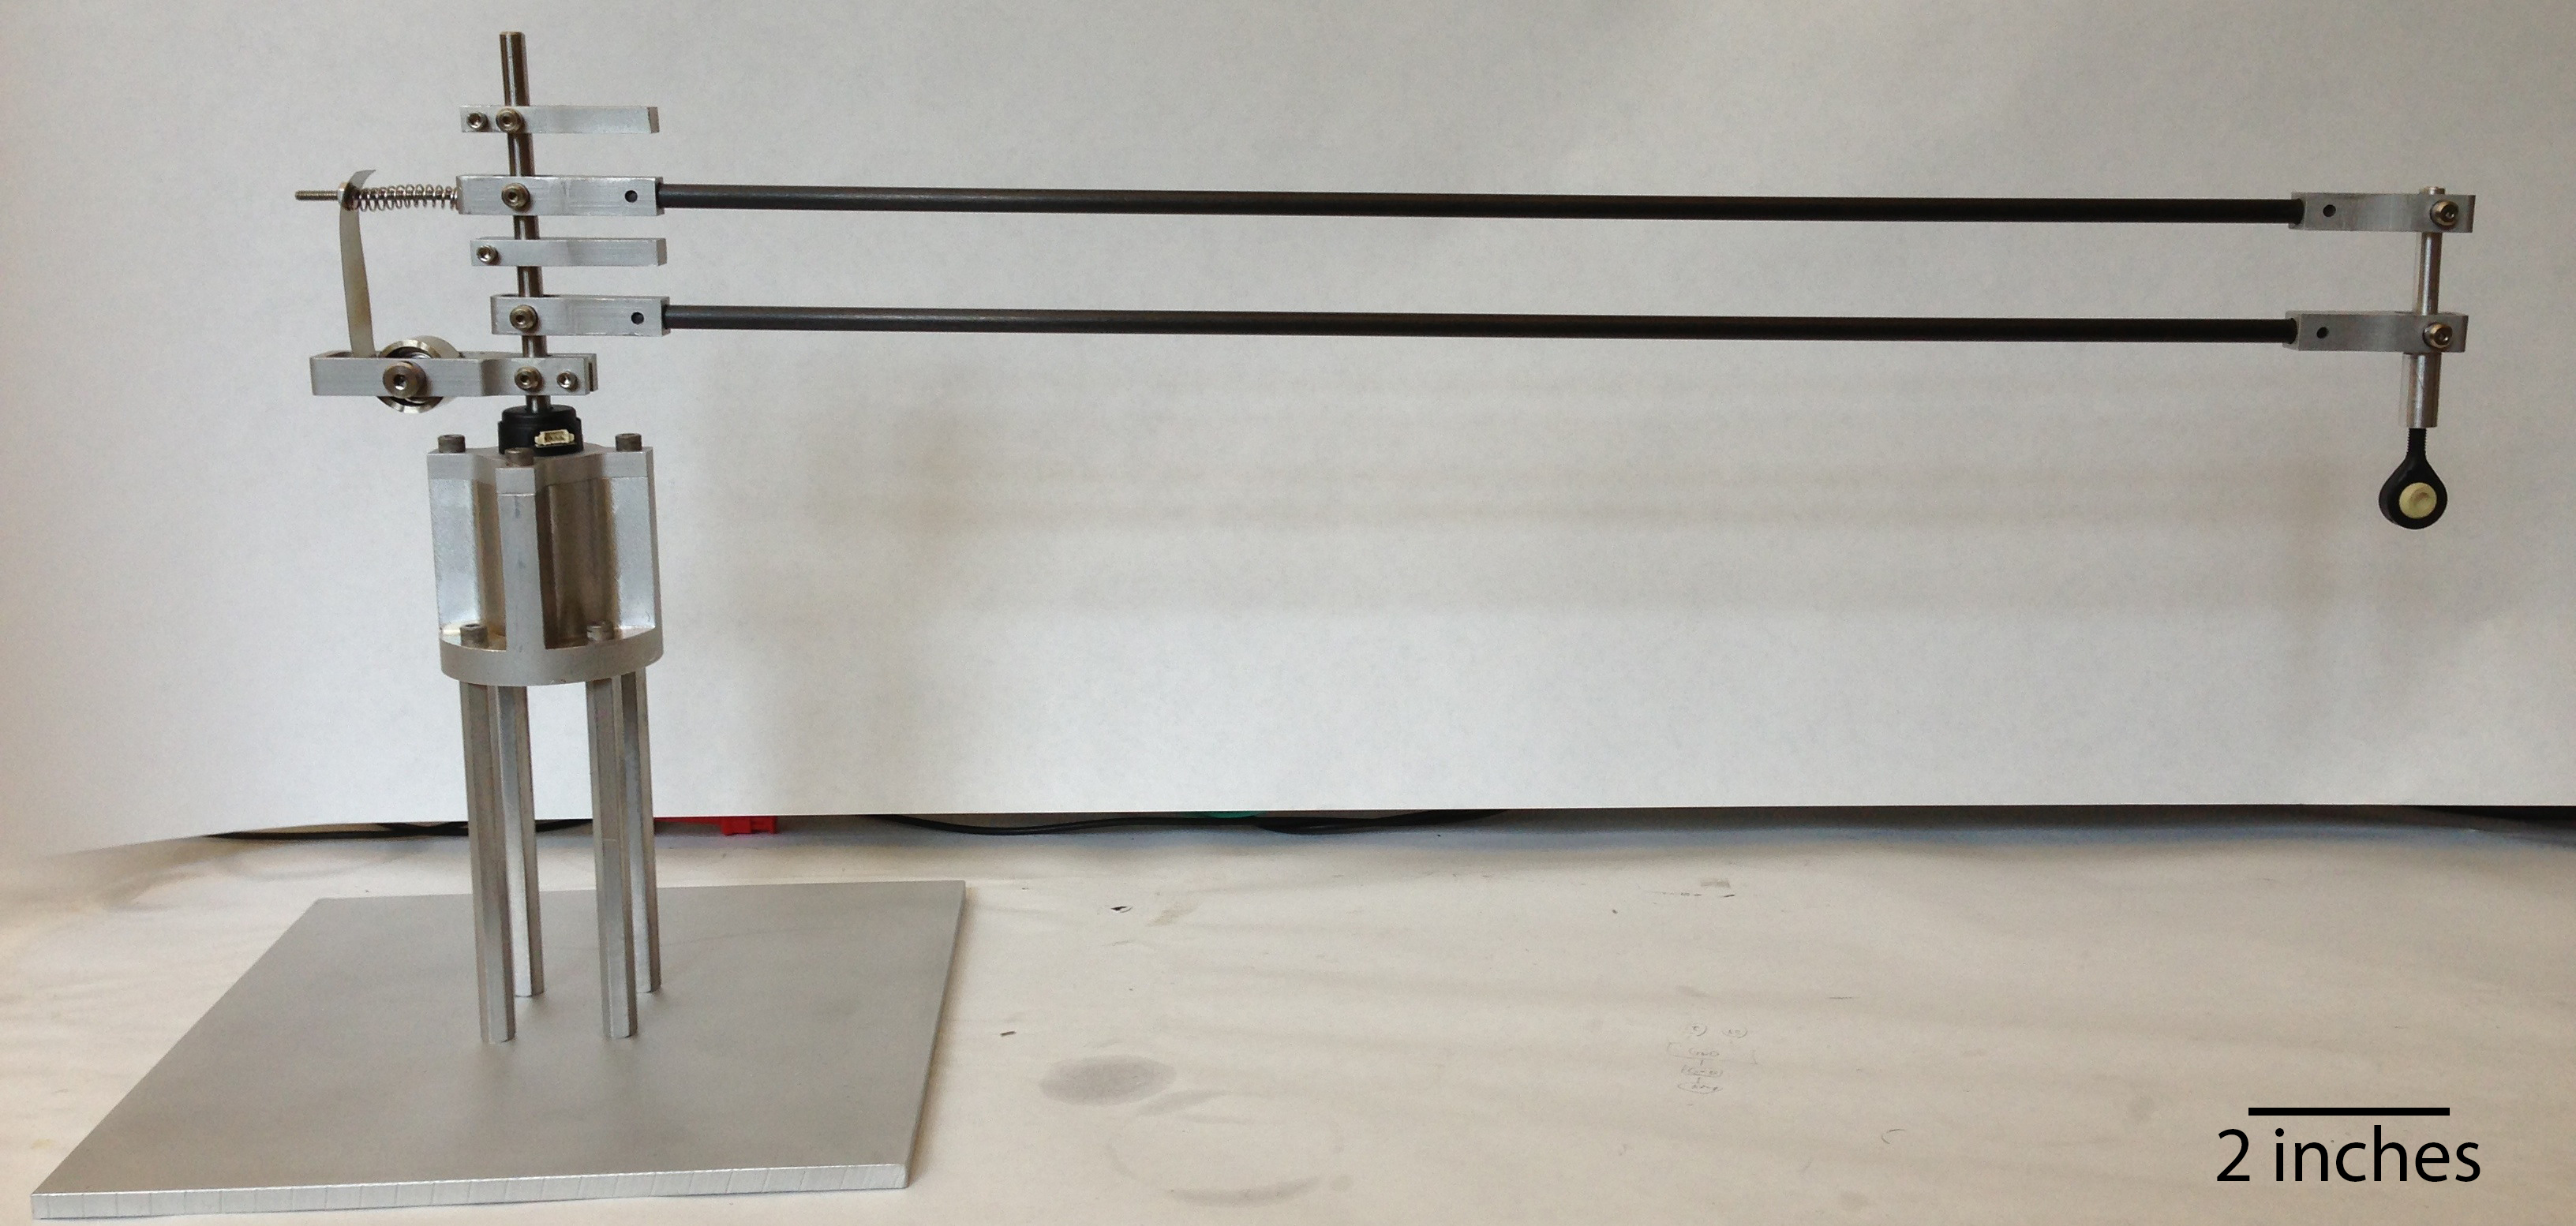
\includegraphics[height = 6in]{boom.jpg}
    \caption{Robot with testing boom (placeholder)}
\end{figure}
\vspace{-1in}
